% +------------------------------------------------------------------------+
% | Reference manual page: HalfedgeDSHalfedge.tex
% +------------------------------------------------------------------------+
% | 22.03.1999   Lutz Kettner
% | Package: HalfedgeDS
% | 
\RCSdef{\RCSHalfedgeRev}{$Revision$}
\RCSdefDate{\RCSHalfedgeDate}{$Date$}
% +------------------------------------------------------------------------+

\ccRefPageBegin

%%RefPage: end of header, begin of main body
% +------------------------------------------------------------------------+


\begin{ccRefConcept}{HalfedgeDSHalfedge}
\label{pageHalfedgeDSItemsHalfedgeRef}

\ccDefinition
  
The concept \ccRefName\ defines the requirements for the local \ccc{Halfedge} 
type in the \ccc{HalfedgeDS} concept. It is also required in 
the \ccc{Halfedge_wrapper<Refs,Traits>} member class template of an
items class, see the \ccc{HalfedgeDSItems} concept.

A halfedge is an oriented edge between two vertices. It is always
paired with a halfedge pointing in the opposite direction. The
\ccc{opposite()} member function returns this halfedge of opposite
orientation. The \ccc{next()} member function points to the successor
halfedge along the face -- or if the halfedge is a border halfedge --
along the open region. A halfedge optionally stores a reference to the
previous halfedge along the face, a reference to an incident vertex,
and a reference to an incident face. Type tags indicate whether the
related member functions are supported.
Figure~\ccTexHtml{\ref{figurePolyOptionalMethods} 
on page \pageref{figureHalfedgeDSOptionalMethods}}{}\begin{ccHtmlOnly}
  <A HREF="#figureHalfedgeDSOptionalMethods"><IMG 
  SRC="cc_ref_up_arrow.gif" ALT="reference arrow" WIDTH="10" HEIGHT="10"></A>
\end{ccHtmlOnly}
depicts the relationship between a halfedge and its incident
halfedges, vertices, and faces.

\begin{ccTexOnly}
    \begin{figure}[bht]
        \begin{center}
          \parbox{\textwidth}{%
              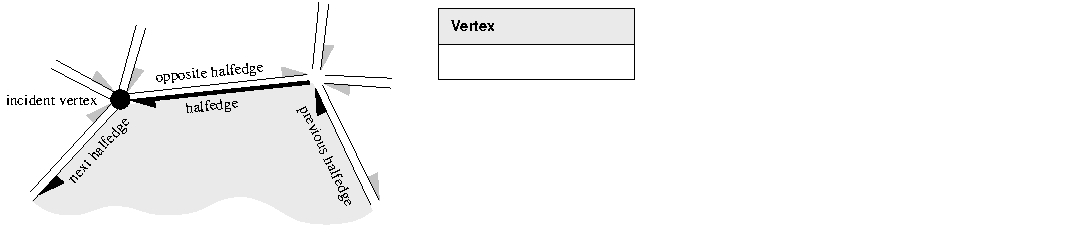
\includegraphics[width=\textwidth]{fig/hds_optional.ips}%
          }
        \end{center}
        \caption{The three classes \protect\ccc{Vertex}, 
          \protect\ccc{Halfedge}, and 
          \protect\ccc{Face} of the halfedge data structure. Member
          functions with shaded background are mandatory. The others
          are optionally supported.}
        \label{figureHalfedgeDSOptionalMethods}
    \end{figure}
\end{ccTexOnly}

\begin{ccHtmlOnly}
    <CENTER>
    <A NAME="figureHalfedgeDSOptionalMethods">
    <A HREF="./hds_optional.gif">
        <img src="./hds_optional_small.gif" 
             alt="Class Diagram"></A><BR>
    <A HREF="./hds_optional.gif">Figure:</A>
    The three classes <I>Vertex</I>, <I>Halfedge</I>, and 
          <I>Face</I> of the halfedge data structure. Member
          functions with shaded background are mandatory. The others
          are optionally supported.
    </CENTER>
\end{ccHtmlOnly}

For the protection of the integrity of the data structure classes such
as \ccc{CGAL::Polyhedron_3} are allowed to redefine the modifying member
functions to be private. In order to make them accessible for the
halfedge data structure they must be derived from a base class
\ccc{Base} where the modifying member functions are still public. Even
more protection is provided for the \ccc{set_opposite()} member
function. The base class \ccc{Base_base} provides access to it.  (The
protection could be bypassed also by an user, but not by accident.)

\ccTypes

\ccThree{Halfedge_const_handle}{v.set_halfedge( Halfedge_handle h);}{}
\ccThreeToTwo

\ccNestedType{HalfedgeDS}
    {instantiated \ccc{HalfedgeDS} ( $\equiv$ \ccc{Refs}).}
\ccGlue
\ccNestedType{Base}{base class that allows modifications.}
\ccGlue
\ccNestedType{Base_base}{base class to access \ccc{set_opposite()}.}
\ccGlue
\ccNestedType{Vertex}{model of \ccc{HalfedgeDSVertex}.}
\ccGlue
\ccNestedType{Face}{model of \ccc{HalfedgeDSFace}.}

\ccNestedType{Vertex_handle}{handle to vertex.}
\ccGlue
\ccNestedType{Halfedge_handle}{handle to halfedge.}
\ccGlue
\ccNestedType{Face_handle}{handle to face.}
\ccGlue
\ccNestedType{Vertex_const_handle}{}
\ccGlue
\ccNestedType{Halfedge_const_handle}{}
\ccGlue
\ccNestedType{Face_const_handle}{}

\ccNestedType{Supports_halfedge_prev}{either \ccc{CGAL::Tag_true} or 
  \ccc{CGAL::Tag_false}.}
\ccGlue
\ccNestedType{Supports_halfedge_vertex}{\~{}}
\ccGlue
\ccNestedType{Supports_halfedge_face}{\~{}}

\ccCreation
\ccCreationVariable{h}

\ccConstructor{Halfedge();}{default constructor.}

\ccOperations
\ccTagFullDeclarations

\ccMethod{Halfedge_handle opposite();}{}
\ccGlue
\ccMethod{Halfedge_const_handle opposite() const;}{the opposite halfedge.}
\ccGlue
\ccMethod{void set_opposite( Halfedge_handle h);}{
    sets opposite halfedge to $h$.}

\ccMethod{Halfedge_handle next();}{}
\ccGlue
\ccMethod{Halfedge_const_handle next() const;}
    {the next halfedge around the face.}
\ccGlue
\ccMethod{void set_next( Halfedge_handle h);}{
    sets next halfedge to $h$.}

\ccMethod{bool             is_border() const;}
    {is true if \ccVar\ is a border halfedge.}

\ccHeading{Operations available if \ccc{Supports_halfedge_prev} $\equiv$ 
           \ccc{CGAL::Tag_true}}

\ccMethod{Halfedge_handle prev();}{}
\ccGlue
\ccMethod{Halfedge_const_handle prev() const;}
    {the previous halfedge around the face.}
\ccGlue
\ccMethod{void set_prev( Halfedge_handle h);}{
    sets prev halfedge to $h$.}

\ccHeading{Operations available if \ccc{Supports_halfedge_vertex} $\equiv$ 
           \ccc{CGAL::Tag_true}}

\ccMethod{Vertex_handle       vertex();}{}
\ccGlue
\ccMethod{Vertex_const_handle vertex() const;}{the incident vertex of \ccVar.}
\ccGlue
\ccMethod{void set_vertex( Vertex_handle v);}{
    sets incident vertex to $v$.}

\ccHeading{Operations available if \ccc{Supports_halfedge_face} $\equiv$ 
           \ccc{CGAL::Tag_true}}

\ccMethod{Face_handle       face();}{}
\ccGlue
\ccMethod{Face_const_handle face() const;}
    {the incident face of \ccVar.  If \ccVar\ is a border halfedge 
      the result is default construction of the handle.}
\ccGlue
\ccMethod{void set_face( Face_handle f);}{
    sets incident face to $f$.}

\ccHasModels

\ccRefIdfierPage{CGAL::HalfedgeDS_halfedge_base<Refs>}\\
\ccRefIdfierPage{CGAL::HalfedgeDS_halfedge_min_base<Refs>}

\ccSeeAlso

\ccRefIdfierPage{HalfedgeDS}\\
\ccRefIdfierPage{HalfedgeDSItems}\\
\ccRefIdfierPage{HalfedgeDSVertex}\\
\ccRefIdfierPage{HalfedgeDSFace}

\end{ccRefConcept}

% +------------------------------------------------------------------------+
%%RefPage: end of main body, begin of footer
\ccRefPageEnd
% EOF
% +------------------------------------------------------------------------+

